\chapter{Examples}
\label{ch:chapter}

\lettrine[lines=\iniciale, slope=0.5em, lraise=0, nindent=1em, findent=-1em]%
{\textcolor{\accentcolor}{A}} nearly full list of features and tools are tested here, from typesetting to citations. \blindtext

\section{Section}

\subsection{Subsection}

\subsubsection{Subsubsection}\marginpar{A `subsubsection' will not appear in the ToC... }

Normal, \textit{italic}, \textbf{bold}, \textbf{\textit{bold-italic}}, UPPERCASE,\textsc{small-capitals}, \textss{superscript}, \hl{highlight}. (If you don't see \emph{small capitals}, your font does not have them).

\noindent Testing characters: 1234567890 .,:;?!``'' @ \# \$ \% \& \* () [] \{\} <> || - -- --- + = * \textbackslash /

\noindent ``Common'' ligatures: ff, fi, and ffi, ``rare'' ones are: st, ct, is. 

\nth{1} \nth{2} \nth{3} \nth{4} \nth{19} century \textsc{bc}, \textsc{ad}.

\section{Typesetting}

\begin{table}
\begin{tabular}{@{}lll@{}}
\toprule
Normal      & Sphinx of black quartz, judge my missing vow forever. \\
Italic      & \textit{Sphinx of black quartz, judge my missing vow forever.} \\
Bold        & \textbf{Sphinx of black quartz, judge my missing vow forever.} \\
Bold-Italic & \textbf{\textit{Sphinx of black quartz, judge my missing vow forever.}} \\
Uppercase   & \uppercase{Sphinx of black quartz, judge my missing vow forever.} \\
Small caps  & \textsc{Sphinx of black quartz, judge my missing vow forever.} \\
Superscript & \textss{Sphinx of black quartz, judge my missing vow forever.} \\
Sans serif  & \textsf{Sphinx of black quartz, judge my missing vow forever.} \\
Mono        & \texttt{Sphinx of black quartz, judge my missing vow forever.} \\ \bottomrule
\end{tabular}
\caption{Different font styles and typefaces.}
\end{table}

\blindtext 

\subsection{Scripts}

Various scripts:

\textbf{Latin}: \tabto{5cm} mitológia

\textbf{Greek}: \tabto{5cm} μυθολογία

\textbf{Cyrillic}: \tabto{5cm} митолоогија 

\textbf{Chinese, Traditional}: \tabto{5cm} 神話。

\textbf{Chinese, Simplified}: \tabto{5cm} \zh{神话。}

\textbf{Japanese}: \tabto{5cm} しんわ

\textbf{Korean}: \tabto{5cm} 신화

\textbf{Arabic}: \tabto{5cm} مِيثُولُوجِيَا

\textbf{Hebrew}: \tabto{5cm} מיתולוגיה

\textbf{Devanagari}: \tabto{5cm} पौराणिक

\textbf{Tibetan}: \tabto{5cm} {\tibetanfont{བར་དོ་ཐོས་གྲོལ}}

% \textbf{Latin}: A a, Á á, B b, C c, Cs cs, D d, Dz dz, Dzs dzs, E e, É é, F f, G g, Gy gy, H h, I i, Í í, J j, K k, L l, Ly ly, M m, N n, Ny ny, O o, Ó ó, Ö ö, Ő ő, P p, Q q, R r, S s, Sz sz, T t, Ty ty, U u, Ú ú, Ü ü, Ű ű, V v, W w, X x, Y y, Z z, Zs zs.

% \textbf{Greek}: Α α, Β β, Γ γ, Δ δ, Ε ε, Ζ ζ, Η η, Θ θ, Ι ι, Κ κ, Λ λ, Μ μ, Ν ν, Ξ ξ, Ο ο, Π π, Ρ ρ, Σ σ/ς, Τ τ, Υ υ, Φ φ, Χ χ, Ψ ψ, Ω ω.

% \textbf{Cyrillic}: A a, Б б, В в, Г г, Д д, Ѓ ѓ, E e, Ж ж, З з, Ѕ ѕ, И и, J j, К к, Л л, Љ љ, М м, Н н, Њ њ, О о, П п, Р р, С с, Т т, Ќ ќ, У у, Ф ф, Х х, Ц ц, Ч ч, Џ џ, Ш ш.

\subsubsection{Bidirectional Scripts}

Arabic and Hebrew in English paragraphs, in mixed environments:

ما هو \foreignlanguage{english}{differentiation}? 

What is ما هو in Arabic?
\medskip
\textnormal
\noindent Most Arabic speakers consider the two varieties to be two registers
of one language, although the two registers can be referred to in
Arabic as فصحى العصر \textit{fuṣḥā l-ʻaṣr} Modern Standard Arabic (MSA) and
فصحى التراث \textit{fuṣḥā t-turāth} Classical Arabic (CA). ʿArab\={i}.

\medskip

The first line of the Bible is בְּרֵאשִׁית בָּרָא אֱלֹהִים אֵת הַשָּׁמַיִם וְאֵת הָאָרֶץ (Genesis 1:1).

% % Actual right-to-left paragraphs (warning).
% \selectlanguage{arabic}
% مكانة عائلته الاجتماعية مكنته من الدراسة على يد أفضل المدرسين في المغرب العربي. تلقى علم التربية الإسلامية التقليدية، ودرس القرآن الكريم الذي كان يحفظه عن ظهر قلب، واللسانيات العربية، وأساس فهم القرآن، الحديث، الشريعة (القانون) والفقه علم التاريخ.
% \selectlanguage{english}

% For inline usage: \foreignlanguage{hebrew}{תַּבְלִין}

\noindent{\color{black}\rule{\linewidth}{0.2mm}} 

\noindent{\color{black}\rule{0.25\linewidth}{0.2mm}} this is baseline

\noindent{\color{black}\rule[0.5ex]{0.25\linewidth}{0.2mm}} this is half raised

\noindent{\color{black}\rule[1ex]{0.25\linewidth}{0.2mm}} this is raised

\noindent{\color{black}\rule[1.5ex]{0.25\linewidth}{0.2mm}} this is raised above

\clearpage

\section{Acronyms, Glossary Terms, and Indexing}

The \hologo{LaTeX} typesetting markup language is specially suitable for documents that are annoying to make.

\bigskip

Glossaries and acronyms both have to be set in the glossary.tex with similar methods, and then called in the text. When an acronym appears for the first time, its full form is also shown. Such as, \gls{OED} but the second time \gls{OED}. For plural and capital glossaries use \gls{taxon} and \glspl{taxon}; \Gls{taxon} and \Glspl{taxon}.

Index one\index{one} is here and \index{other one} two\index{two} is here. There is also index for tables \index{three|tb}, figures\index{four|fg}, and footnotes\index{five|fn}.
Also, there is grouped indexing possible for things like black pepper\index{pepper!black}, white pepper\index{pepper!white}, and green pepper\index{pepper!green}. 

% WARNING: The index on Overleaf only prints on your pdf if you run it for the first time/clear the cache. I don't know why, currently unsolved.

\section{Citations}

Citation examples, such as \autocite[99]{laufer_sino-iranica_1919}, which now is the same as \parencite[99]{laufer_sino-iranica_1919} and \textcite{laufer_sino-iranica_1919}, but footcite also exists.\footcite{laufer_sino-iranica_1919} 
Multi-volume citing is also available, \pvolcite[]{9}[99]{ei2} \& \tvolcite[]{9}[99]{ei2}.

\section{Lists and Environments}
\label{sec:environments}

\begin{enumerate}
    \item one
    \item two
    \item three
\end{enumerate}

\begin{itemize}
    \item one
    \item two
    \item three
\end{itemize}

\begin{note}
    This is a note.
\end{note}

\begin{equation}
    \label{eq:1}
    x^2  = 1
\end{equation}

This (above) is an equation. In Equation \ref{eq:1} we have~$\sqrt{\log n}$.

\ex
\begingl
\gla\rightcomment{Hungarian (Finno-Ugric, \emph{reference})}Ez egy nyelvészeti példamondat.//
\glb This a linguistic example-sentence//
\glft ``This is a linguistic example sentence.''//
\endgl
\xe

\begin{etymology}\label{etym:pepper}
\raggedright
English \textit{pepper}
< Middle English \textit{peper}
< Old English \textit{pipor}
< West Germanic \textit{*piper}
< Latin \textit{piper} `black pepper, long pepper'
< Ancient Greek \textit{péperi} `pepper'
< Pahlavi
< Middle Indo-Aryan \textit{pipparī} `long pepper'
< Sanskrit \textit{pippalī} `berry, peppercorn', \textit{pippali} `long pepper'\footnote{This is a custom, iterating environment that you can modify for whatever purpose.}
\end{etymology}

This line has a reference for Etymology \ref{etym:pepper} and a `clever reference' for \Cref{sec:environments}. And below is a quote.

\epigraph{By convention sweet and by convention bitter, by convention hot, by convention cold, by convention color; but in reality atoms and void.}{Democritus, \nth{3} century BC\\(DK 68B9, trans. Taylor 1999a)}

\blindtext

\section{Figures}

\begin{figure}
    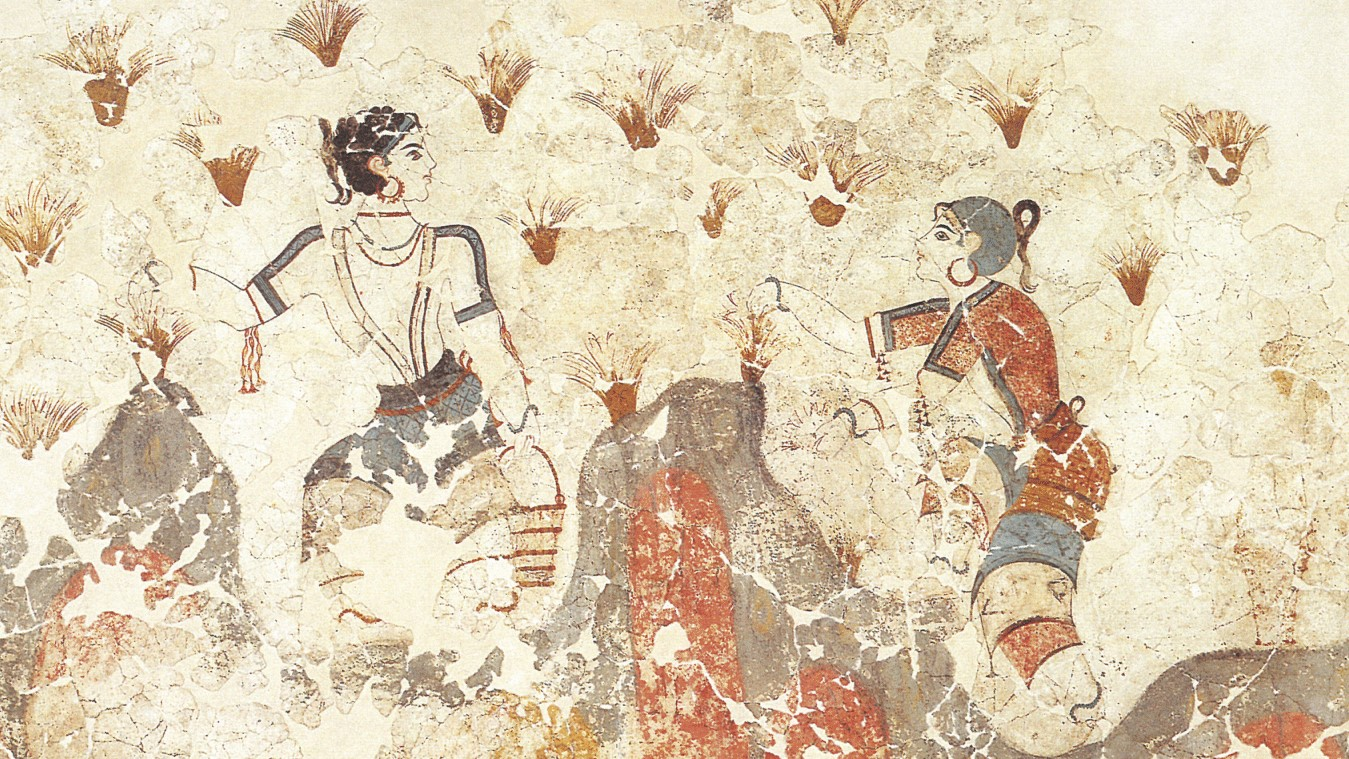
\includegraphics[width=\linewidth]{imgs/saffron_gatherers.jpg}
    \caption[Short caption to ToC]{Long caption}
    \label{fig:saffron1}
\end{figure}

\todo{Place figures better}

\begin{figure}[!hbt]
    \centering
    \subfloat{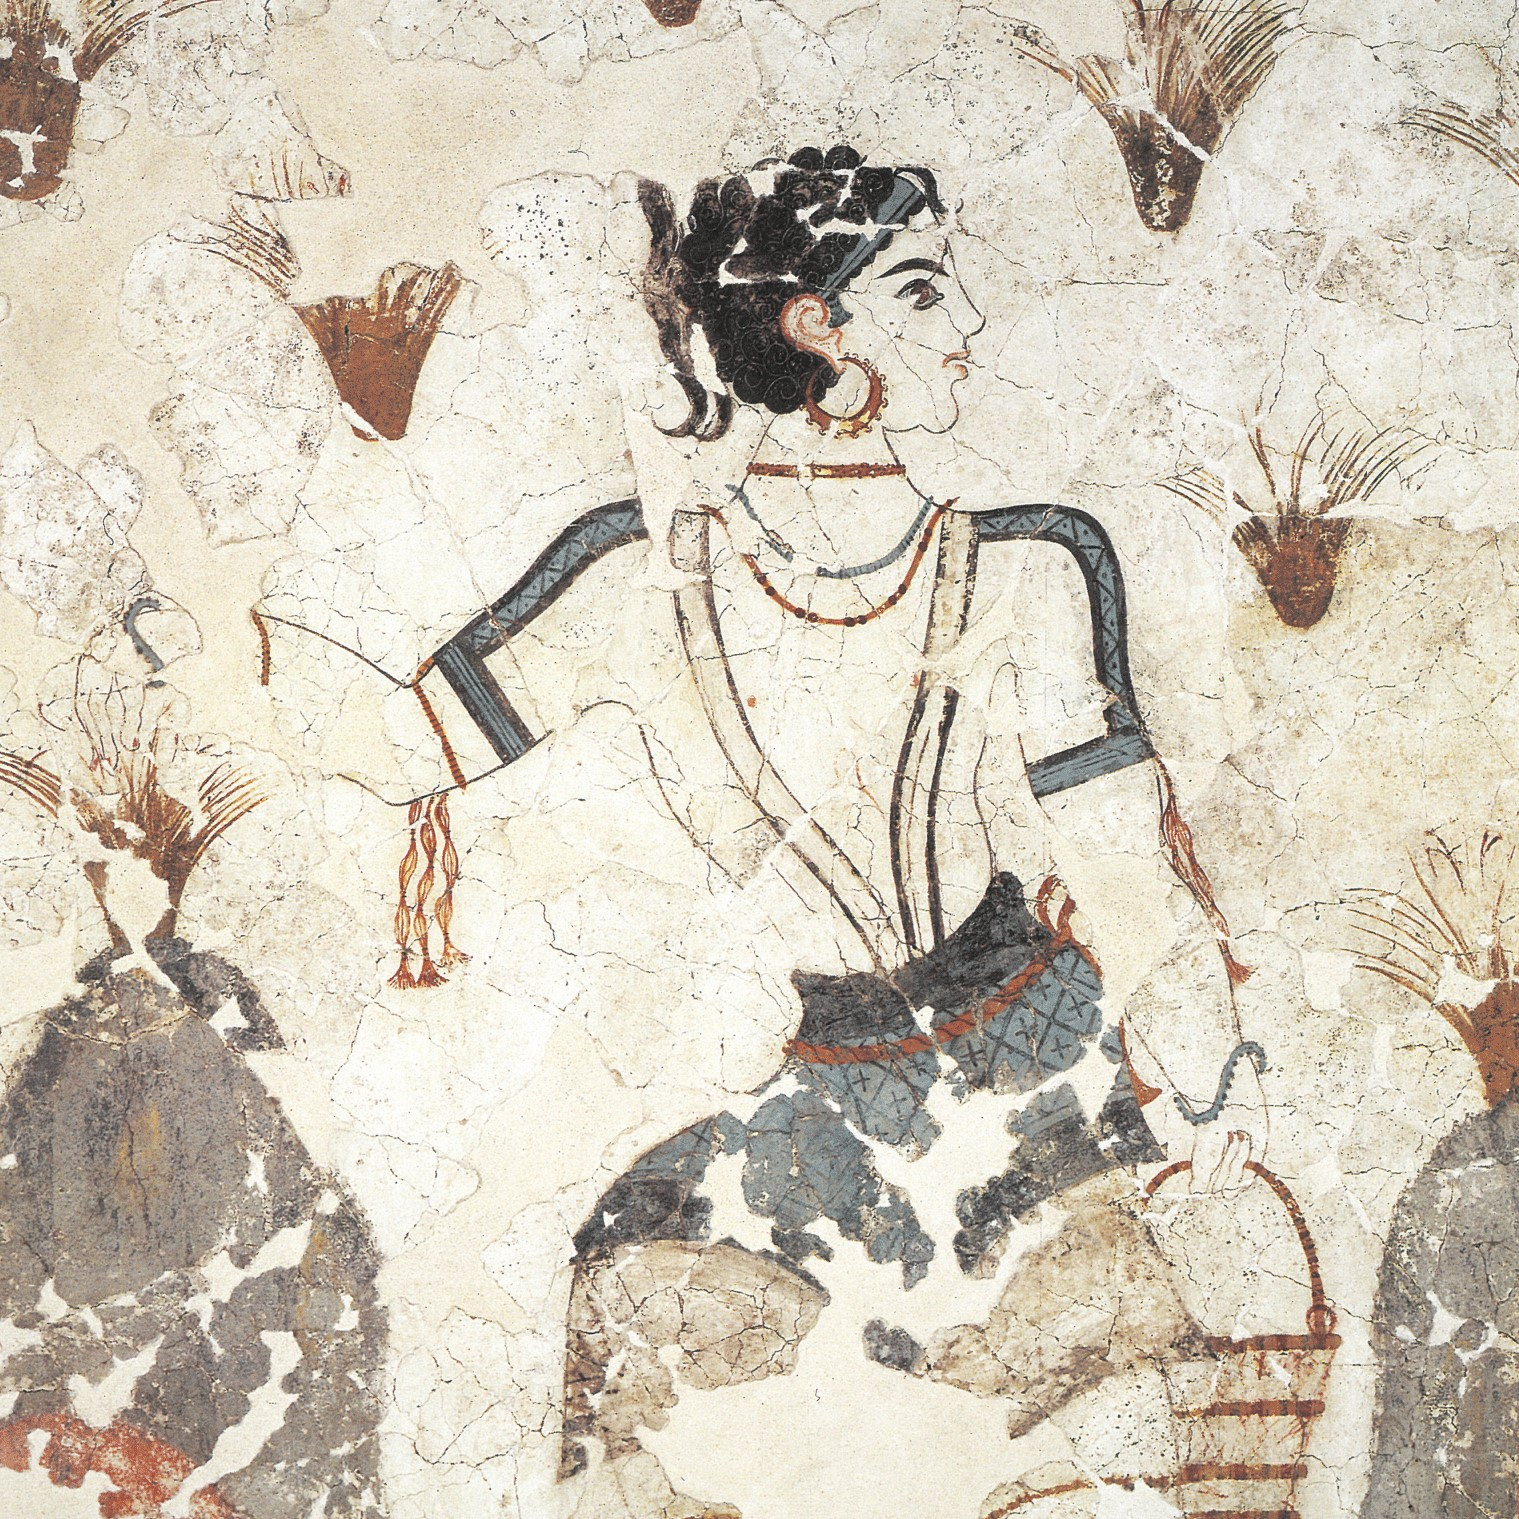
\includegraphics[width=0.482\linewidth]{imgs/saffron_gatherers_l.jpg}}
    \hfill
    \subfloat{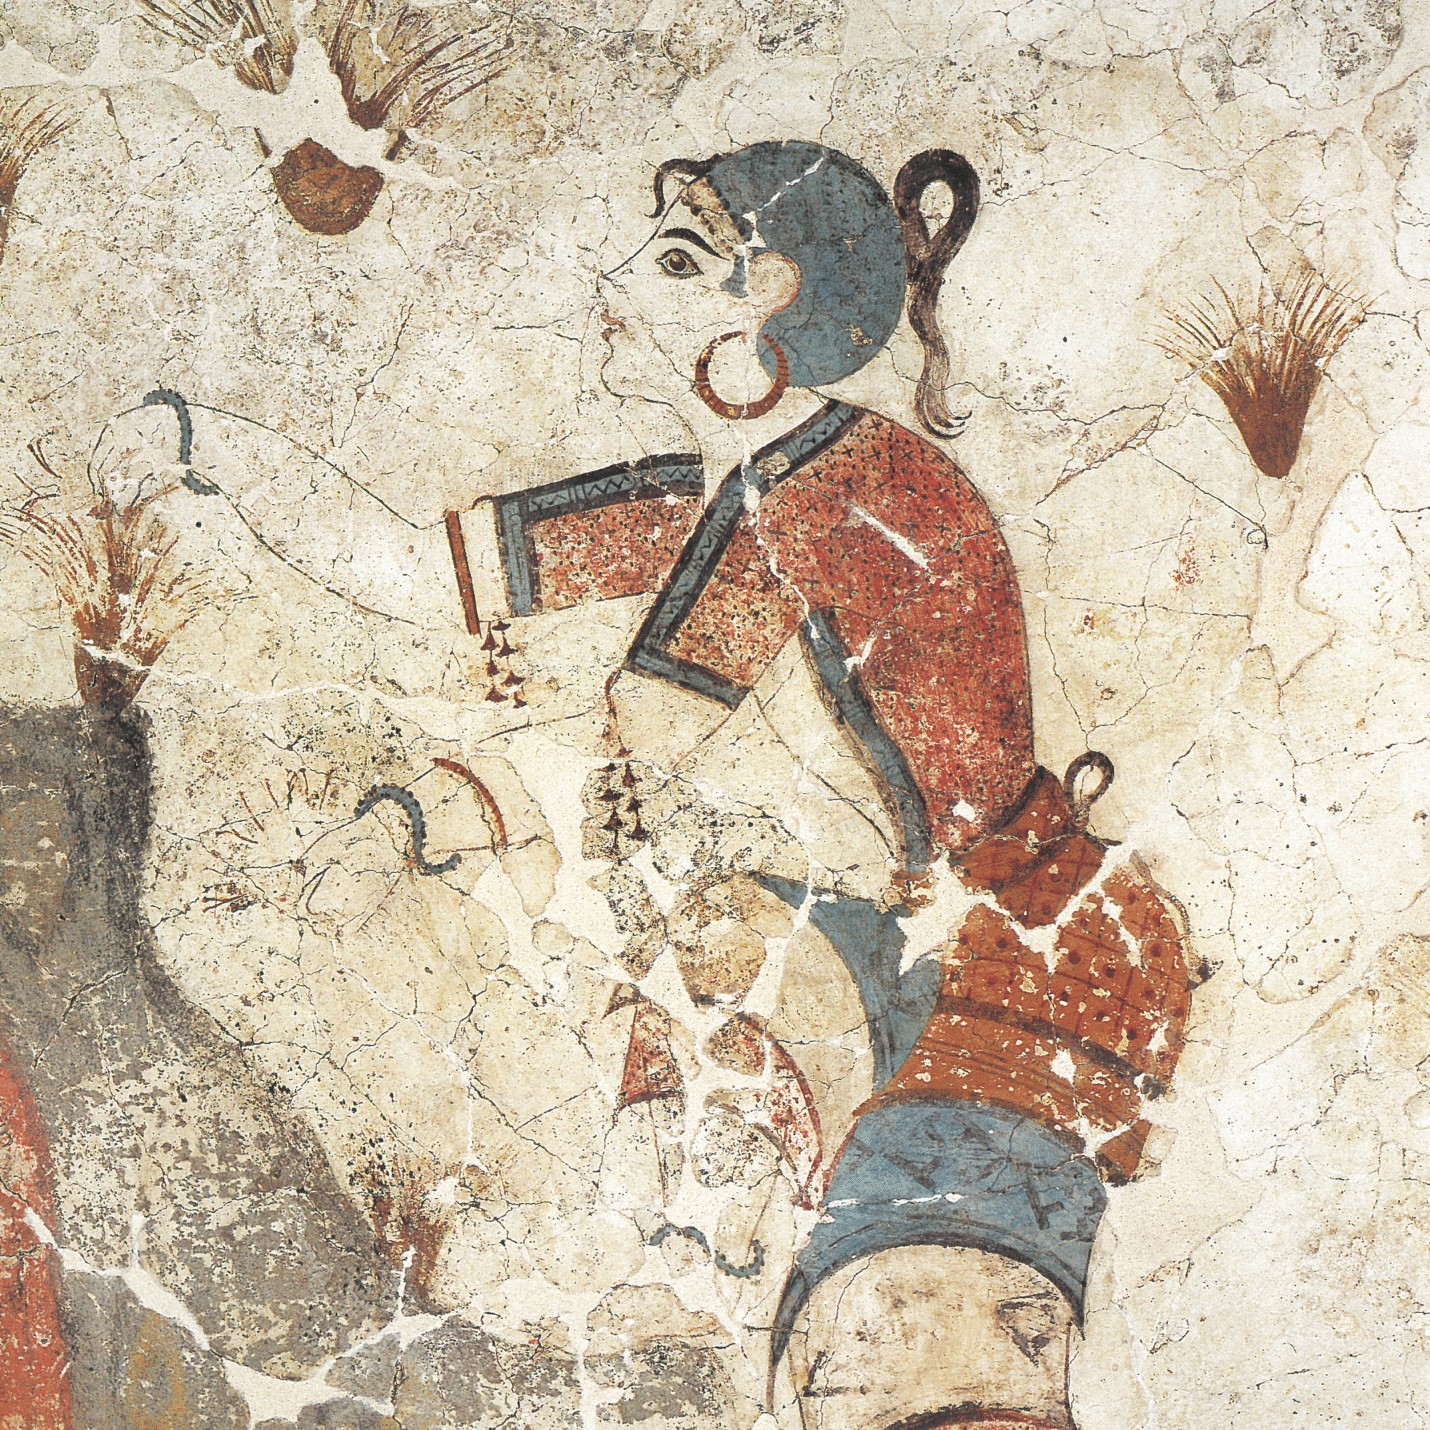
\includegraphics[width=0.482\linewidth]{imgs/saffron_gatherers_r.jpg}}
    \caption[Saffron-gatherers]{Saffron-gatherers; details from the mural on the east wall in room 3a, first floor, at Xeste 3 site, Akrotiri at Thera \autocite[152]{doumas_wall-paintings_1992}.}
    \label{fig:saffron2}
\end{figure}

\blindtext

\section{Trees}

\begin{center}
\begin{forest}
    for tree={align=center}
    [paprika\\\small{English}
    [paprika\\\small{Hungarian} 
    [pàprika\\\small{Serbian-Croatian-Bosnian} 
    [*pĭpĭrĭ\\\small{Proto-Slavic} 
    [piper\\\small{Latin} 
    [péperi\\\small{Ancient Greek},name=AG 
    [*\\\small{Pahlavi} 
    [pipparī\\\small{Middle Indo-Aryan} 
    [pippalī\\\small{Sanskrit}]]]]]] 
    [piperi\\\small{Modern Greek},edge=dashed,name=MG]]]]
    \draw[-] (AG.north) to (MG.south);
    \draw[->,dotted] (AG) to[out=east,in=south] (MG);
\end{forest}
\begin{tabular}[t]{ll@{}}
\tikz[baseline]\draw(0,1ex)--(1,1ex); & borrowed\\
\tikz[baseline]\draw[dotted](0,1ex)--(1,1ex); & descended\\
\tikz[baseline]\draw[dashed](0,1ex)--(1,1ex); & influenced\\
\end{tabular}
\end{center}

\blindtext


\section{Tables}

\setlength{\tabcolsep}{3pt} % Change separator length

\begin{table}[ht]
% \begin{adjustbox}{max width=\textwidth}
\begin{tabularx}{\textwidth}{@{}r>{\footnotesize}llll@{}rl@{}}
\toprule
\textbf{\#} & \multicolumn{1}{l}{\textbf{Species}} & \textbf{English} & \textbf{Chinese} & \textbf{Translit.} & \textbf{Arabic} & \textbf{Translit.}     \\ \midrule
1           & \textit{Pimenta dioica}            & allspice         & 多香果              & \textit{duōxiāngguǒ}     & فلفل إفرنجي     & \textit{filfil ifranjī}      \\
2           & \textit{Pimpinella anisum}         & anise            & 茴芹               & \textit{huíqín}          & ينسون           & \textit{yansūn}              \\
3           & \textit{Ferula assa-foetida} et al.& asafoetida       & 阿魏               & \textit{āwèi}            & حلتیت           & \textit{ḥiltīt}              \\
4           & \textit{Carum carvi}               & caraway          & 葛縷子              & \textit{gělǚzi}          & كراويا          & \textit{karāwiyā}            \\
5           & \textit{Elettaria cardamomum}      & cardamom         & \tc{荳蔻}            & \textit{dòukòu}          & هال             & \textit{hāl}                 \\
6           & \textit{Cinnamomum cassia}         & cassia           & 肉桂               & \textit{ròuguì}          & سليخة           & \textit{salīkha}             \\
7           & \textit{Capsicum annuum} et al.    & chile            & 辣椒               & \textit{làjiāo}          & فلفل حار        & \textit{fulful hārr}         \\
8           & \textit{Cinnamomum verum}          & cinnamon         & 錫蘭肉桂             & \textit{xīlánròuguì}     & قرفة            & \textit{qirfa}               \\
9           & \textit{Syzygium aromaticum}       & clove            & 丁香               & \textit{dīngxiāng}       & قرنفل           & \textit{qaranful}            \\
10          & \textit{Coriandrum sativum}        & coriander        & \tc{芫荽}               & \textit{yánsui}          & كزبرة           & \textit{kuzbara}             \\
11          & \textit{Cuminum cyminum}           & cumin            & 孜然               & \textit{zīrán}           & كمون            & \textit{kammūn}              \\
12          & \textit{Anethum graveolens}        & dill             & 蒔蘿               & \textit{shíluó}          & شبت             & \textit{shibitt}             \\
13          & \textit{Foeniculum vulgare}        & fennel           & 茴香               & \textit{huíxiāng}        & شمر             & \textit{shamar}              \\
14          & \textit{Trigonella foenum-graecum} & fenugreek        & 胡蘆巴              & \textit{húlúbā}          & حلبة            & \textit{ḥulba}               \\
15          & \textit{Zingiber officinale}       & ginger           & 薑                & \textit{jiāng}           & زنجبيل          & \textit{zanjabīl}            \\
16          & \textit{Piper longum}              & long pepper      & 蓽撥               & \textit{bìbō}            & دار فلفل        & \textit{dār filfil}          \\
17          & \textit{Myristica fragrans}        & mace             & \tc{肉荳蔻皮}             & \textit{ròudòukòupí}    & بسباسة	& \textit{basbāsa} \\
18          & \textit{Myristica fragrans}        & nutmeg           & \tc{肉荳蔻}          & \textit{ròudòukòu}       & جوز الطيب       & \textit{jawz al-ṭīb}         \\
19          & \textit{Piper nigrum}              & pepper           & 胡椒               & \textit{hújiāo}          & فلفل            & \textit{filfil, fulful}      \\
20          & \textit{Crocus sativus}            & saffron          & 番紅花              & \textit{fānhónghuā}      & زعفران          & \textit{zaʿfarān}            \\
21          & \textit{Zanthoxylum spp.}          & Sichuan pepper   & 花椒               & \textit{huājiāo}         & فلفل سيتشوان    & \textit{filfil sītshuwān}    \\
22          & \textit{Illicium verum}            & star anise       & 八角               & \textit{bājiǎo}          & ينسون نجمي      & \textit{yansūn najmī}        \\
23          & \textit{Curcuma longa}             & turmeric         & 薑黃               & \textit{jiānghuáng}      & كركم            & \textit{kurkum}              \\
24          & \textit{Vanilla planifolia}        & vanilla          & 香草               & \textit{xiāngcǎo}        & فانيليا         & \textit{fānīliyā}\\ 
\midrule
 & & & & & & \\ \midrule
25          & \textit{Physeter macrocephalus*} & ambergris        & 龍涎香              & \textit{lóngxiánxiāng}   & عنبر            & \textit{ʿambar}          \\
26          & \textit{Cinnamomum camphora}     & camphor          & 樟                & \textit{zhāng}           & كافور           & \textit{kāfūr}           \\
27          & \textit{Moschus moschiferus*}    & musk             & 麝香               & \textit{shèxiāng}        & مسك             & \textit{misk}            \\
28          & \textit{Boswellia sacra}         & frankincense     & 乳香               & \textit{rǔxiāng}         & لبان            & \textit{lubān}           \\
29          & \textit{Commiphora myrrha}       & myrrh            & 沒藥               & \textit{mòyào}           & مر              & \textit{murr}            \\
30          & \textit{Santalum album}          & santalwood       & 旃檀               & \textit{zhāntán}         & الصندل          & \textit{ṣandal}          \\ 
\bottomrule
\end{tabularx}
% \end{adjustbox}
\caption[An elaborate table]{The set of 24 spices included in this thesis, with scientific names of the source plant, names in English, Chinese, Arabic, and their transliterations.}
\label{table:set}
\end{table}

\setlength{\tabcolsep}{6pt} % Default separator length

\blindtext

\section{IPA}

\textipa{[ðIsIzsAmaIpeI]}, \textipa{[Its\*rilijizitutaIp]} as in: ``This is some IPA, it's really easy to type.''

\begin{longtable}{p{0.15\textwidth}p{0.3\textwidth}p{0.3\textwidth}}
  \toprule
  \endfirsthead
  \toprule
  \endhead
  \bottomrule
  \endfoot
  \bottomrule
  \endlastfoot
  Consonant & Onset & Coda\tabularnewline

  \midrule p & pun.za (claw) & \textipa{k\super hap.Ra} (old man)\tabularnewline

  b & \textipa{bO\|[d\super h} (bull) & \textipa{Seb.Ra} (dull)\tabularnewline

  \textipa{b\super h} & \textipa{b\super he\:d} (sheep) & \tabularnewline

  m & \textipa{mE} (me) & \textipa{amb} (mango)\tabularnewline

  f & ful (flower) & \tabularnewline

  \textipa{V} & \textipa{Vi\|[d.jaR.\|[t\super hi} & \textipa{RoVa}
  (injury)\tabularnewline

  \textipa{\|[t} & \textipa{\|[tu} (you) & \textipa{mO\|[t}
  (don't)\tabularnewline

  \textipa{\|[d} & \textipa{\|[deS} (many) & \textipa{swa\|[d}\tabularnewline

  \textipa{\|[t\super h} & \textipa{\|[t\super he\:n.\:di} (cold) &
  \textipa{hO\|[t\super h} (hand)\tabularnewline

  \textipa{\|[d\super h} & \textipa{\|[d\super hus.ki} (down) &
  \textipa{bO\|[d\super h} (bull)\tabularnewline

  \textipa{\t*{ts}} & \textipa{\t*{ts}Ol.\:na} (to walk) & \textipa{so\t*{ts}}
  (think)\tabularnewline

  \textipa{\t*{ts}\super h} & \textipa{\t*{ts}\super hekke} (fast) &
  \tabularnewline

  \textipa{\t*{dz}} & \textipa{\t*{dz}a.\:na} (to go) & \tabularnewline

  \textipa{n} & \textipa{n@i} (no) & \textipa{an.\|[dRe} (inside)\tabularnewline

  \textipa{R} & \textipa{me.Ri} (my) & \textipa{g\super hOR}\tabularnewline

  \textipa{s} & \textipa{sen.\|[tRi} (orange colour) & \textipa{hOs\:na} (to
  laugh)\tabularnewline

  \textipa{z} & \textipa{ze\:d} (root) & \textipa{Roz} (everyday)\tabularnewline

  \textipa{l} & \textipa{lOm.ma} (long) & \textipa{kal}
  (yesterday)\tabularnewline

  \textipa{S} & \textipa{Sob.la} (beautiful) & \textipa{gaS}
  (rain)\tabularnewline

  \textipa{\:t} & \textipa{\:te\:d.\:da} (curved) & \textipa{nO\:t.\:t\super he}
  (gone)\tabularnewline

  \textipa{\:t\super h} & \textipa{\:t\super he\:n\:ra} (cold) &
  \textipa{nO\:t.\:t\super he} (gone)\tabularnewline

  \textipa{\:d} & & \textipa{ne\:d} (near)\tabularnewline

  \textipa{\:d\super h} & & \textipa{pO\:d\super h.na} (to read)\tabularnewline

  \textipa{\:r} & \textipa{pO\:ru} (fell) & \textipa{me\:n.\:r\super h@k}
  (frog)\tabularnewline

  \textipa{\:n} & \textipa{\|[de.\:na} (to give) & \textipa{ku\:n}
  (who)\tabularnewline

  \textipa{\:l} & \textipa{ke\:la} (banana) & \tabularnewline

  \textipa{\t*{tS}} & \textipa{\t*{tS}Ok.ku\|[da} (rotten) & \tabularnewline

  \textipa{\t*{dZ}} & \textipa{\t*{dZ}epuR} (Jaipur) & \tabularnewline

  \textipa{j} & \textipa{ja\|[d} (remember) & \textipa{gaj}
  (abuse)\tabularnewline

  \textipa{k} & \textipa{ki.\:ra} (snake) & \textipa{b\super huk}
  (hunger)\tabularnewline

  \textipa{g} & \textipa{ga} (cow) & \textipa{b\super hEg.\:na} (to
  run)\tabularnewline

  \textipa{k\super h} & \textipa{k\super ha\:na} (to eat) & \textipa{paNk\super
    h} (wing)\tabularnewline

  \textipa{g\super h} & \textipa{g\super hOR} (house) & \tabularnewline

\end{longtable}

\section{Notes}

A thesis submitted for examination purpose should include the words ‘Initial Submission for Examination Purpose’ lettered on the front cover. For details, see: this link \url{https://www.polyu.edu.hk/gs/rpghandbook/ref-regulations-format-thesis/} or the \href{https://www.polyu.edu.hk/gs/rpghandbook/section10/}{RPg Handbook}
Transliteration of Arabic script: \href{https://referenceworks.brillonline.com/pages/help/transliteration-islam}{Brill Online}

The original of this LaTeX template was created by Tom M. Ragonneau (https://github.com/ragonneau/phd-thesis-template). I have modified it for linguistics-oriented theses.